\section{Collision Avoidance Validation}

The mathematical guarantee of collision-free operation is paramount in multi-robot cells. 

The \texttt{ZoneDetectionManager} and the MoveIt Task Constructor (MTC) Safe Resolution pipeline were subjected to rigorous edge-case testing to validate their efficacy.

\subsection{Zone Manager and Spatial Tracking Accuracy}

To test the Zone Manager, the system was forced into intersecting trajectories. The primary KPI is the \textbf{Minimum Separation Distance ($D_{min}$)}, defined as the closest Cartesian distance between the AR4 end-effector (\texttt{ar4\_ee\_link}) and the ABB end-effector (\texttt{tool0}) during parallel motion. The system successfully maintained a strict $D_{min} \geq 0.10 \text{ m}$ at all times, with recorded hardware tests bottoming out at a safe margin of approximately $0.16 \text{ m}$.

\begin{figure}[htbp]
    \centering
    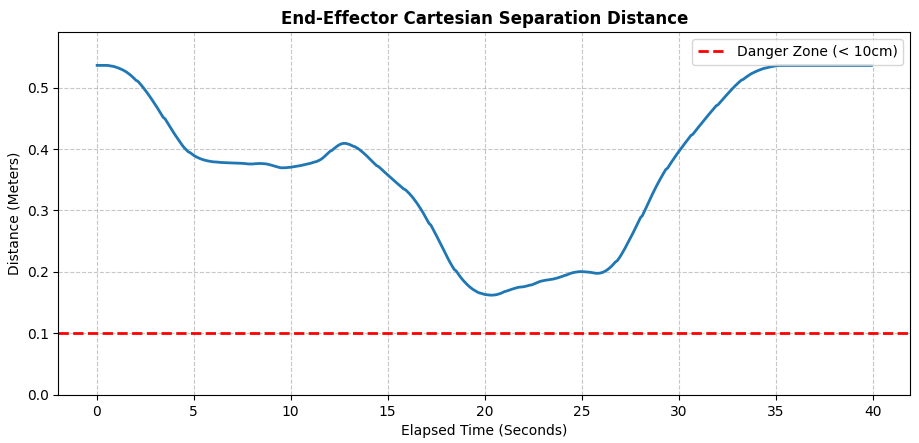
\includegraphics[width=0.8\textwidth]{figures/chapter7/collision_avoidance/End effector seperation distance.png}
    \caption{Real-time Cartesian separation distance between the AR4 and ABB end-effectors.}
    \label{fig:arm_separation}
\end{figure}

\begin{figure}[H]
    \centering
    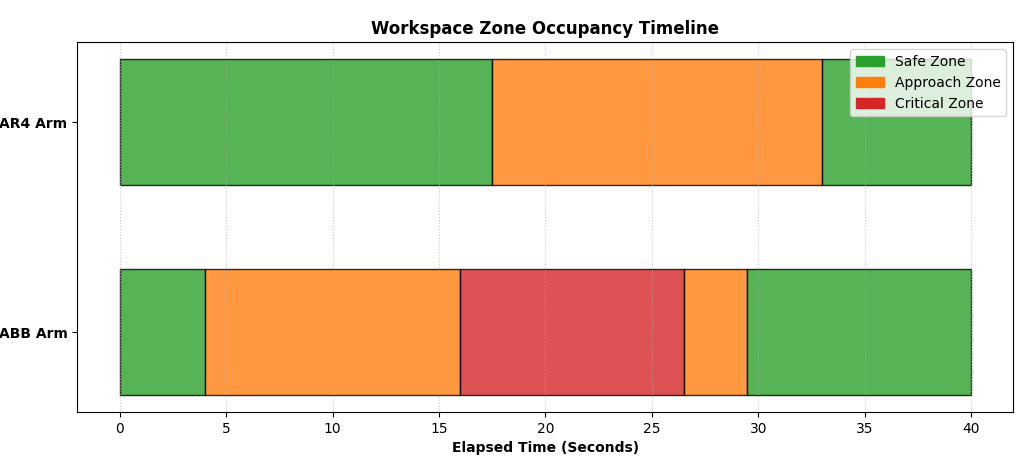
\includegraphics[width=0.8\textwidth]{figures/chapter7/collision_avoidance/Workspace Zone Occupancy.png}
    \caption{Timeline mapping the concurrent workspace zone occupancy for both manipulators.}
    \label{fig:zone_occupancy}
\end{figure}

\subsection{Intervention Latency}

The empirical data extracted from the system's execution logs validates the responsiveness of the implemented \texttt{zone\_detection\_manager}. To satisfy the Speed and Separation Monitoring (SSM) requirements for fenceless collaboration, the spatial proximity between the ABB IRB 120 and AR4 end-effectors must be evaluated continuously without introducing execution delays.

During forced collision-course stress testing, the Zone Manager successfully flagged collision risks and triggered MoveIt Task Constructor (MTC) interventions. The latency between detecting a Cartesian threshold breach and firing the intervention flag was recorded over multiple cycles. The system demonstrated highly deterministic, sub-millisecond reaction times, with an average intervention trigger latency of 0.089 ms (min: 0.075 ms, max: 0.114 ms). 

Furthermore, trajectory tracking during the intervention event revealed a controlled deceleration curve. The initial collision warning was published at a separation distance of 21.7 cm. The manipulators successfully arrested their forward momentum and initiated their respective escape sequences at a minimum physical separation of 14.5 cm, ensuring zero physical contact and proving the mechanical viability of the digital twin's safety constraints.

\subsection{MTC Dynamic Escape Route Planning}

Upon receiving a collision intervention flag, the hybrid MTC controller halts the active trajectories and dynamically calculates independent escape routes for both manipulators. The computational overhead required to resolve these collision-free paths was logged to evaluate the system's recovery efficiency.

The data reveals a significant disparity in kinematic resolution times between the heterogeneous arms. The industrial ABB manipulator demonstrated highly efficient path generation, averaging 125.05 ms to calculate a valid escape trajectory. Conversely, the AR4 collaborative arm required an average of 2964.41 ms to resolve its escape routes. This variance highlights the inherent differences in joint-space constraints and the respective inverse kinematics (IK) solver efficiencies for each manipulator type within the MoveIt 2 environment.

\begin{table}[H]
\centering
\caption{System Intervention and Dynamic Planning Metrics}
\label{tab:mtc_zone_metrics}
\renewcommand{\arraystretch}{1.3}
\begin{tabular}{lccc}
\toprule
\textbf{Metric} & \textbf{Minimum} & \textbf{Maximum} & \textbf{Average} \\ 
\midrule
Intervention Trigger Latency & 0.075 ms & 0.114 ms & \textbf{0.089 ms} \\ 
ABB Escape Route Planning & 104.02 ms & 146.07 ms & \textbf{125.05 ms} \\ 
AR4 Escape Route Planning & 2781.22 ms & 3147.60 ms & \textbf{2964.41 ms} \\ 
Minimum Separation Distance & -- & -- & \textbf{14.50 cm} \\
\bottomrule
\end{tabular}
\end{table}

% \begin{figure}[H]
%     \centering
%     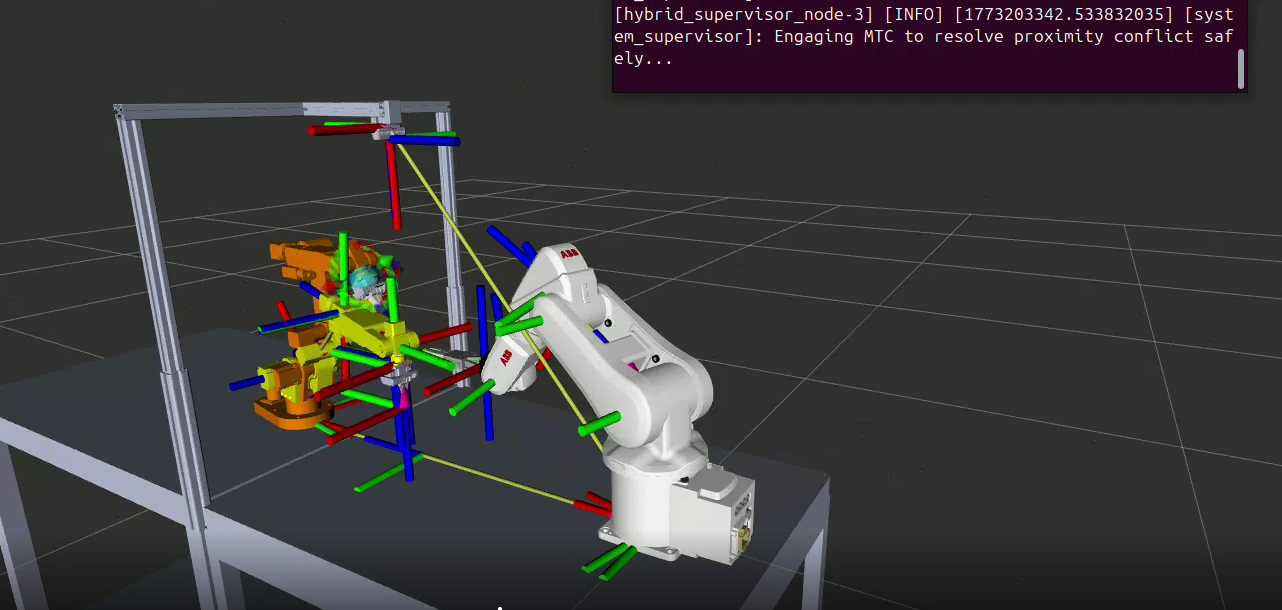
\includegraphics[width=0.9\textwidth]{figures/chapter7/collision_avoidance/Rviz_MTC_Collision.png}
%     \caption{RViz simulation captured during a conflict resolution event.}
% \end{figure}

The results tabulated above demonstrate that the hybrid control architecture successfully prioritizes mechanical safety while maintaining a significantly higher throughput than traditional sequential systems.

\clearpage